\documentclass[crop,tikz]{standalone}
\usetikzlibrary{backgrounds}
\colorlet{blue}{cyan}
\tikzset{
  inverted/.style = {
    every path/.style = {draw=white,text=white},
    background rectangle/.style={fill},
    show background rectangle
  }
}

\tikzset{>=latex}

\begin{document}
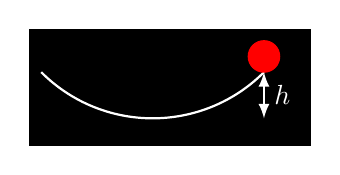
\begin{tikzpicture}[inverted,inverted]
  \pgfmathsetmacro{\angl}{45}
  \pgfmathsetmacro{\radius}{2}
  \pgfmathsetmacro{\circleRadius}{0.2}
  \coordinate (ball) at (-\angl:\radius);
  % track
  \draw[thick] (ball) arc (-\angl:-180+\angl:\radius);
  % ball
  \draw[fill,red] (ball)+(0,\circleRadius) circle (\circleRadius);
  % height
  \draw[<->,thick] (ball) -- node[right] {$h$} ++(0,{\radius*(-1+cos(\angl))});
\end{tikzpicture}%
\end{document}
